%%%%%%%% ICML 2019 EXAMPLE LATEX SUBMISSION FILE %%%%%%%%%%%%%%%%%

\documentclass{article}

% Recommended, but optional, packages for figures and better typesetting:
\usepackage{microtype}
\usepackage{graphicx}
% \usepackage{subfigure}
\usepackage{booktabs} % for professional tables
\usepackage{soul}

\usepackage{makecell}
\usepackage{circuitikz}
\usepackage{caption}
\usepackage{subcaption}
\usepackage{graphicx}
\usepackage{amsmath}

% hyperref makes hyperlinks in the resulting PDF.
% If your build breaks (sometimes temporarily if a hyperlink spans a page)
% please comment out the following usepackage line and replace
% \usepackage{icml2019} with \usepackage[nohyperref]{icml2019} above.
\usepackage{hyperref}

\renewcommand{\vec}[1]{\mathbf{#1}} % re-style the vector
\usepackage{tikz}
\usetikzlibrary{
  arrows.meta, % for Straight Barb arrow tip
  fit, % to fit the group box around the central neurons
  positioning, % for relative positioning of the neurons
}

% Attempt to make hyperref and algorithmic work together better:
\newcommand{\theHalgorithm}{\arabic{algorithm}}

% Use the following line for the initial blind version submitted for review:
\usepackage[accepted]{icml2019}

% If accepted, instead use the following line for the camera-ready submission:
%\usepackage[accepted]{icml2019}

\def\layersep{2.5cm}

\tikzset{
  neuron/.style={ % style for each neuron
    circle,draw,thick, % drawn as a thick circle
    inner sep=0pt, % no built-in padding between the text and the circle shape
    minimum size=3.5em, % make each neuron the same size regardless of the text inside
    node distance=2em and 4em, % spacing between neurons (y and x)
  },
  group/.style={ % style for the groups of neurons
    rectangle,draw,thick, % drawn as a thick rectangle
    inner sep=0pt, % no padding between the node contents and the rectangle shape
  },
  output/.style={ % style for the inputs/outputs
    neuron, % inherit the neuron style
    fill=gray!15, % add a fill color
  },
  input/.style={ % style for each neuron
    circle%,draw,thick, % drawn as a thick circle
    inner sep=0pt, % no built-in padding between the text and the circle shape
    minimum size=2.5em, % make each neuron the same size regardless of the text inside
    node distance=2em and 4em, % spacing between neurons (y and x)
  },
  conn/.style={ % style for the connections
    -{Straight Barb[angle=60:2pt 3]}, % simple barbed arrow tip
    thick, % draw in a thick weight to match other drawing elements
  },
}

% The \icmltitle you define below is probably too long as a header.
% Therefore, a short form for the running title is supplied here:

% XXX Potentially get rid of "Deep"
\icmltitlerunning{Can Inter-layer Recurrent Neural Networks Learn Algorithms?}

\begin{document}

\twocolumn[
% XXX Potentially get rid of "Deep"
% XXX Potentially talk about algorithm learning, program synthesis
\icmltitle{Can Inter-layer Recurrent Neural Networks Learn Algorithms?}

% It is OKAY to include author information, even for blind
% submissions: the style file will automatically remove it for you
% unless you've provided the [accepted] option to the icml2019
% package.

% List of affiliations: The first argument should be a (short)
% identifier you will use later to specify author affiliations
% Academic affiliations should list Department, University, City, Region, Country
% Industry affiliations should list Company, City, Region, Country

% You can specify symbols, otherwise they are numbered in order.
% Ideally, you should not use this facility. Affiliations will be numbered
% in order of appearance and this is the preferred way.
\icmlsetsymbol{equal}{*}

\begin{icmlauthorlist}
\icmlauthor{Anthony Proschka}{can}
\end{icmlauthorlist}

\icmlaffiliation{can}{Candis GmbH, Berlin, Germany}

\icmlcorrespondingauthor{Anthony Proschka}{anthony@candis.io}

% You may provide any keywords that you
% find helpful for describing your paper; these are used to populate
% the "keywords" metadata in the PDF but will not be shown in the document
\icmlkeywords{Machine Learning, ICML}

\vskip 0.3in
]

% this must go after the closing bracket ] following \twocolumn[ ...

% This command actually creates the footnote in the first column
% listing the affiliations and the copyright notice.
% The command takes one argument, which is text to display at the start of the footnote.
% The \icmlEqualContribution command is standard text for equal contribution.
% Remove it (just {}) if you do not need this facility.

%\printAffiliationsAndNotice{}  % leave blank if no need to mention equal contribution
\printAffiliationsAndNotice{} % otherwise use the standard text.

\begin{abstract}
While recurrent neural networks have been proven to express universal Turing machines, \textit{training} them to perform arbitrary computable functions exactly is difficult. In this paper, we introduce a novel architecture called Inter-layer Recurrent Neural Network (ILRNN, pronounced "iLearn"), a form of deep recurrent neural network that exhibits extended and top-down connectivity across layers. Despite being inspired by both biological neural networks and digital circuit design, we cannot yet show that an ILRNN using conventional optimization techniques learns to add arbitrarily large binary numbers (not even with informed initial hyperparameter configuration). It remains to be evaluated whether a learning algorithm exists that can reliably find global minima in such a network that represent the exact solution and generalize to arbitrarily large binary numbers.

% \begin{itemize}
%     \item and show that there exists a configuration of parameters and hyperparameters that solves the given task exactly. However, we only succeed in training the architecture to solve the task exactly in a small share of trials, despite testing various settings for the activation function and its gradient, the training objective (and regularization), the optimization algorithm and its hyperparameters (such as the learning rate)
%     % pronounced /aɪlɜːn/)
% \end{itemize}
\end{abstract}

\section{Introduction \& Motivation}
\label{motivation}

In recent years, deep learning has shown remarkable progress in applications such as image recognition \cite{NIPS2012_4824}, speech recognition \cite{graves2013speech}, games \cite{mnih2015human, 44806} and photorealistic image generation \cite{goodfellow2014generative}, either being the first technology to ever solve a problem or achieve human parity on it.

% Despite these successes, deep neural networks and the current means to train them still face an array of difficulties: sample complexity, overfitting, and the convergence to potentially useful yet imperfect solutions. \hl{XXX}.

In this paper, we want to draw the attention to three core aspects of the study of artificial neural networks: expressivity, learnability and interpretability.

An important distinction that needs to be made is the fundamental difference between the expressivity of a deep learning model and its learnability. In the realm of real functions, several theoretical works have shown that feed forward artificial neural networks act as universal function approximators, i.e. under certain conditions functions of the form

% $$
% \overset{n}{\underset{k=0}\bigcirc}\ \sigma(W_kx)
% $$

% Incorrect in the sense that I now only have one scalar per layer
% $$
% \overset{n}{\underset{k=0}\bigcirc}\ \sigma(\sum_i^{| l_k |} w_{ki}x_i)
% $$

$$
FNN(x) = (\overset{n}{\underset{k=1}\bigcirc}\ f_k)(x),
$$
$$
\text{where} \  f_k(x) = \sigma(W_k x),
$$

% Note that i shall not forget the bias terms here

$\bigcirc$ is the repeated function composition operator, $n$ is the number of layers, $\sigma$ is the activation function, $W_k \in \mathbb{R}^{l_k \times l_{k-1}}$ is the weight matrix of layer $k$ and $l$ holds the number of neurons for each layer, are able to approximate up to some tolerated error any arbitrary function \cite{cybenko1, hornik1989multilayer, hornik1991approximation}. In the realm of theory of computation, Siegelmann and Sontag have shown that recurrent neural networks are able to simulate any Turing machine, which is equivalent to saying they can compute any partial recursive function (\citeyear{siegelmann1995computational}). Universal function approximation and Turing completeness are structurally different properties and should not be equated. However, they both illustrate that given the right set of hyperparameters and a viable weight configuration, artificial neural networks should in theory be able express a solution to a broad class of tasks. Whether the function that the human brain computes falls into this class is still unclear.

While expressivity seems to be a well established property of ANNs, their learnability is much less so. An early work showed that under certain circumstances, even the smallest networks are NP-hard to train 
% (\hl{It's more about deciding whether there exists an exact solution for a given set of training samples? But they also mention that choice of hyperparameters is important})
\cite{blum1989training}. In most scenarios, the system of polynomial or nonlinear equations resulting from modelling a given set of labelled data using a neural network cannot easily be solved analytically. Other solution and optimization techniques seem to have little guarantees that they find any solution or a global optimum. % (\hl{???}).

Finally, ANNs are still mostly considered "black box" functions that lack interpretability.
% (\hl{XXX})
Once trained to perform a specific task, it is not straightforward to reconstruct what features (with semantic human understandable value) caused a certain prediction or decision, especially when the input features themselves mark low-level entities such as pixels in images or sound frequencies in audio streams. This paper also aims to provide an intuitive understanding of what type of computation is happening in the newly described recurrent neural network architecture.

% \begin{itemize}
%     \item Biological plausibility: not really, since it's unlikely that biological neurons really have logic gate behavior, right?
%     \item But: my approach suggests that - in artificial neural networks -
%     \item We of course somewhat get rid of this whole hierarchical representations topic
% \end{itemize}

Our contributions include the following:
\begin{itemize}
    \item We introduce a novel architecture for deep recurrent neural networks   called inter-layer recurrent neural networks (ILRNN). These networks exhibit extended and top-down connectivity across time steps without introducing cyclical paths in the computational graph. 
    \item Building on top of well-known insights that neural networks can compute logic gates, we show by an example that recurrent neural networks can in fact represent any Boolean circuit perfectly. Thusly, ANNs with the appropriate activation functions can be interpreted as trainable versions of combinational logic.
    \item Formulating a (almost) memoryless binary addition task, we provide an interesting test bed for future work exploring means to teach computational tasks to neural networks.
    \item Using various of today's solving and optimization techniques, we obtain the empirical result that finding the weight configuration that solves the task perfectly is hard.
\end{itemize}

\section{Related Work}
\label{related-work}

In the following section we quickly recap important milestones in the advancements of recurrent neural networks (RNNs) and in the attempts to teach neural networks to learn exact and general solutions to algorithmic and computational problems.

\subsection{Recurrent neural networks}

Rumelhart et al. were possibly the first researchers to study recurrent neural networks (RNNs) as an extension of standard feedforward neural networks with the intention to model sequence and especially time series data (\citeyear{rumelhart1986learning}). They show how their then-novel backpropagation algorithm could be applied to RNNs by unrolling the net for a finite number of time steps and backpropagating error gradients through these.

Around the same time, Jordan publishes a report on using RNNs for sequence modeling \citeyear{jordan1997serial}. There, he also introduces simple nets that have recurrent connections feeding the outputs of a previous time step back to the hidden nodes of the next (note this is a first record of the idea generalized by ILRNNs that will be introduced later in this paper).

One of the major advances in RNN research is the long short-term memory or LSTM cell \cite{hochreiter1997long}. By incorporating gating mechanisms to an RNN cell, they circumvent the so-called vanishing or exploding gradient problem that arises when gradients are backpropagated through many layers of neurons in conventional networks \cite{hochreiter1991untersuchungen, hochreiter2001gradient}. LSTMs and similar models such as GRUs are today widely used in practice \cite{cho2014learning, DBLP:journals/corr/abs-1801-01078}.

In more recent times, several studies have examined RNNs and methods to train them in greater detail. Graves gives thorough explanations on the different types of sequence labeling tasks that can be modelled using RNNs in the supervised setting both when input and output sequences are aligned or not (\citeyear{graves2012supervised}). In his doctoral thesis, Sutskever puts specific emphasis on the problem of properly training RNNs, and provides updates to the model, a second-order optimization algorithm as well as a new initialization scheme \cite{Sutskever:2013:TRN:2604780}. This is particularly interesting for this paper as he recognizes the difficulty of finding a desired solution in an RNN for a given task. 

Deep RNNs, RNNs that have multiple recurrent layers (or cells) stacked on top of each other, were first used to improve the state of the art in speech recognition \cite{graves2013speech}. More specifically, the connectivity across neurons and layers in deep RNNs can be structured in a variety of ways proposed by Pascanu et al. (\citeyear{pascanu2013construct}).

% Since the beginning of artificial neural network research it has been tried to have ANNs learn 

% \begin{itemize}
%     \item \textit{Separate subsection for theoretical foundations (incl. Turing completeness) of RNNs?}
%     \item From a theoretical perspective (which is of particular interest for this paper), Siegelman und Sontag proved that specific instantiations of recurrent neural networks are Turing complete(?) (\citeyear{siegelmann1995computational})
%     \item Do universal approximator theorems of FNNs also hold for RNNs? Are RNNs a special case of FNNs?
%     \item Here we argue/propose/suggest that the community (should) renew its interest in the computational foundations of artificial neural networks as there exist fundamental issues/shortcomings/constraints that block the advancement of general artificial intelligence
%     \item \textit{Cite Grefenstette's summer school talk on RNNs and automata theory}
%     \item Grefenstette argues that RNNs when trained approximate rather FSMs(?) than Turing machines and proposes that RNNs be split into controller and memory modules (as many modern approaches implement, cf. NTM etc.). But this leads to the question: how does the biological brain do this split, and does it to it at all? How does the biological brain store memories if not in its connection weights?
%     \item
% \end{itemize}

\section{Model Definition}

\begin{figure}[!h]
\centering
\begin{tikzpicture}
  % current time step
  \node[output] (yt) {$\vec{y}_t$};
  \node[neuron,below=2em of yt] (htn) {$h_t^n$};
%   \node[neuron,below=of htn] (htm) {$...$};
  \node[neuron,below=3em of htn] (ht1) {$h_t^1$};
  % \node[group,fit={(htn) (htm) (ht1)}] (gr1) {};
  \node[input,below=2em of ht1] (xt) {$\vec{x}_t$};

  \draw[conn] (htn) -- (yt);
%   \draw[conn] (htm) -- (htn);
  \draw[conn] (ht1) -- (htn) node[fill=white, anchor=center, pos=0.5] {...};
  \draw[conn] (xt) -- (ht1);
%   \foreach \destination in {htn,htm,ht1} { % the for loop idea can be expanded to draw the entire diagram quickly
%     \draw[conn] (ht-1n.east) -- (\destination.west);
%   }
  
  % next time step
  \node[neuron,right=of htn] (ht+1n) {$h_{t+1}^n$};
%   \node[neuron,right=of htm] (ht+1m) {$...$};
  \node[neuron,right=of ht1] (ht+11) {$h_{t+1}^1$};
  \node[output,above=2em of ht+1n] (yt+1) {$\vec{y}_{t+1}$};
  \node[input,below=2em of ht+11] (xt+1) {$\vec{x}_{t+1}$};
  
  \draw[conn] (ht+1n) -- (yt+1);
%   \draw[conn] (ht+1m) -- (ht+1n);
  \draw[conn] (ht+11) -- (ht+1n) node[ fill=white, anchor=center, pos=0.5] {...};
  \draw[conn] (xt+1) -- (ht+11);

  \foreach \source in {yt, htn, ht1} {
    \foreach \destination in {yt+1, ht+1n, ht+11} {
      \draw[conn] (\source.east) -- (\destination.west);
    }
  }

  % previous time step
  \node[neuron,left=of htn] (ht-1n) {$h_{t-1}^n$};
%   \node[neuron,left=of htm] (ht-1m) {$...$};
  \node[neuron,left=of ht1] (ht-11) {$h_{t-1}^1$};
  \node[output,above=2em of ht-1n] (yt-1) {$\vec{y}_{t-1}$};
  \node[input,below=2em of ht-11] (xt-1) {$\vec{x}_{t-1}$};
  
  \draw[conn] (ht-1n) -- (yt-1);
%   \draw[conn] (ht-1m) -- (ht-1n);
  \draw[conn] (ht-11) -- (ht-1n) node[fill=white, anchor=center, pos=0.5] {...};
  \draw[conn] (xt-1) -- (ht-11);

  \foreach \source in {yt-1, ht-1n, ht-11} {
    \foreach \destination in {yt, htn, ht1} {
      \draw[conn] (\source.east) -- (\destination.west);
    }
  }
\end{tikzpicture}
\caption{Visualization of ILRNN}
\label{ilrnnviz}
\end{figure}

We consider deep RNNs \cite{graves2013speech}. In the novel architecture called inter-layer recurrent neural networks (ILRNNs), we now extend deep RNN's connectivity in such a way that both the hidden and output units receive incoming connections from all hidden and output units of the previous time step like so:

\[
h_t^n = \sigma(W_{h^{n-1} h^n} h_t^{n-1} + \sum_i W_{h^i,h^n}^r h_{t-1}^i + b_h^n),
\]

where $h_t^i$ is the hidden activation at time step $t \in \{0, ..., T\}$ and hidden layer $i \in \{1, ..., N\}$, $W$ is the set of feedforward weight matrices, $W^r$ is the set of recurrent weight matrices, $b_h^i$ is the bias vector for hidden layer $i$ and $\sigma$ is an arbitrary activation function.

Figure~\ref{ilrnnviz} shows the connectivity between the different hidden layers across time steps graphically. Note that the output layer is considered the final hidden layer in this notation. Also note that despite top-down connections between layers, since they occur across time steps no cyclical paths on the computational graph are added (allowing this architecture to be trained with conventional BPTT). While this increases the number of free parameters compared to the standard deep RNN considerably, this increase still fares well in comparison with converting a simple RNN cell to an LSTM cell. Surprisingly, to our knowledge this is the first paper to introduce this specific connectivity in recurrent neural networks.

This architecture is a general case of the net by Siegelman & Sontag to prove their computational power (\citeyear{siegelmann1995computational}). It should thus exhibit the same guarantees in terms of expressivity.

\section{Task Description}

This section describes a specific formulation of the binary addition task that was used to evaluate both the expressibility and learnability of ILRNN.

As outlined in Section~\ref{related-work}, considerable previous work has been done to enable ANNs to learn algorithmic tasks, programs and other programming language related problems. A popular sample task is \textit{addition}. A variety of different formulations for the addition task exist, differing in the choice of numbering system (binary vs. decimal), encoding scheme (raw vs. one-hot encoding), model type (feedforward vs. recurrent) and external devices (none vs. scratchpad etc.) (cf. \citealt{npi}).

The literature most relevant to this paper has one trait in common: it uses large recurrent models (at times augmented with external memory devices) and formulates addition in a way that requires the model to memorize or actively read the entire sequence of addends before it outputs its result. This is where the binary addition task deployed differs with its predecessors: ILRNN is fed one pair of addends per time step, and can immediately output its corresponding sum. The only information it has to keep track of across time (and thus using its memory capabilities) is the potential carry that can result from the sum of two individual digits. A step-by-step illustration that deduces the representation fed to ILRNN from the original written base-10 addition that humans learn during elementary school is depicted in Table~\ref{sample-table}.

The procedure used to generate a sample of a given sequence length is depicted in Algorithm~\ref{alg:binary-addition}. Its assignment statements for $y_1$ and $carry$ prove interesting because these are exactly the set of expressions we wish ILRNN to internalize. We are effectively nudging the neural network to express Boolean algebra through its neural pathways.

One advantage of this task is that it naturally provides out-of-sample  instances that can be used to test generalization: simply evaluate the trained model on adding numbers that are larger, i.e. have more digits than the ones seen during training. While our approach does not require the model to hold increasingly large binary numbers in memory, it simply evaluates whether the network is able to learn the exact addition logic needed to add arbitrarily large binary numbers. Ideally this addition logic is not degraded through spurious information passed through recurrent connections as the numbers become larger.


\begin{table*}[t]
\caption{Different representations of the addition task}
\label{sample-table}
\vskip 0.15in
\begin{center}
\begin{small}
\begin{sc}
\begin{tabular}{lcccr}
\toprule
Decimal addition & Binary addition & \makecell{Binary addition \\ (reverse order)} & \makecell{Network inputs \& targets (over time)} \\
\midrule
\makecell{ \texttt{\ \ 387} \\ \texttt{+\ \ 18} \\ \texttt{= 405} } & \makecell{ \texttt{\ \ 110000011} \\ \texttt{+\ 000010010} \\ \texttt{=\ 110010101} } & \makecell{ \texttt{\ \ 110000011} \\ \texttt{+\ 010010000} \\ \texttt{=\ 101010011} } & 
\begin{tabular}{cccccccccc}
     & $t_1$ & $t_2$ & $t_3$ & $t_4$ & $t_5$ & $t_6$ & $t_7$ & $t_8$ & $t_9$ \\
    $x_1$ &\texttt{1} & \texttt{1} & \texttt{0} & \texttt{0} & \texttt{0} & \texttt{0} & \texttt{0} & \texttt{1} & \texttt{1} \\
    $x_2$ & \texttt{0} & \texttt{1} & \texttt{0} & \texttt{0} & \texttt{1} & \texttt{0} & \texttt{0} & \texttt{0} & \texttt{0} \\
    $y_1$ & \texttt{1} & \texttt{0} & \texttt{1} & \texttt{0} & \texttt{1} & \texttt{0} & \texttt{0} & \texttt{1} & \texttt{1} \\
\end{tabular} \\
\bottomrule
\end{tabular}
\end{sc}
\end{small}
\end{center}
\vskip -0.1in
\end{table*}

% [tb] parameter apparently causes algorithm to be top of column
\begin{algorithm}[tb]
   \caption{Generate binary addition sample}
   \label{alg:binary-addition}
\begin{algorithmic}
   \STATE {\bfseries Input:} maximum digits per addend $n$, 
   % \REPEAT
   \STATE Initialize $carry = false$, $sample = []$
   % $x_1 = $, $x_2 = $.
   \FOR{$i=1$ {\bfseries to} $n$}
   \STATE Draw $x_1$, $x_2$ uniformly from $\{0, 1\}$
%   \IF{$carry == false$}
   \STATE $y_1 = (x_1 \oplus x_2) \oplus carry$
   \STATE $carry = x_1 \land x_2 + carry \land (x_1 \oplus x_2)$
%   \ELSE
%   \STATE \hl{$y_1 = XXX$, $carry = XXX$}
%   \ENDIF
   \STATE Append $(x_1, x_2, y_1)$ to $sample$
   \ENDFOR
   \IF{$carry == true$}
   \STATE Append $(0,0,1)$ to $sample$
   \ENDIF
   \STATE Return $sample$
   % Should this algorithm be a generator? But isn't generator something
   % Python specific? So many we don't even use the REPEAT here?
   % \UNTIL{$noChange$ is $true$}
   % \RETURN $sample$
\end{algorithmic}
\end{algorithm}

\section{Experiments}

After introducing a new recurrent neural network model and specifying a specific form of binary addition task, the results of the experiments are reported. It is important to note that no experiment reported in this paper was conducted without incorporating prior knowledge into the model architecture. Accordingly, first the manual construction or rather deduction of the hyperparameter settings will be explained, before the attempt for an analytic solution and the training procedure using an gradient descent algorithm.

% \begin{figure*}[t]
% \begin{center}

% \begin{subfigure}[t]
% \begin{circuitikz} \draw
% (0,2) node[and port] (myand1) {}
% (0,0) node[and port] (myand2) {}
% (2,1) node[xnor port] (myxnor) {}
% (myand1.out) -- (myxnor.in 1)
% (myand2.out) -- (myxnor.in 2);
% \end{circuitikz}
% \end{subfigure}

% % \begin{subfigure}[t]
% % \begin{circuitikz} \draw
% % (0,2) node[and port] (myand1) {}
% % (0,0) node[and port] (myand2) {}
% % (2,1) node[xnor port] (myxnor) {}
% % (myand1.out) -- (myxnor.in 1)
% % (myand2.out) -- (myxnor.in 2);
% % \end{circuitikz}
% % \end{subfigure}

% \end{center}
% \end{figure*}

% \begin{figure*}[t]
% % \centering
% \begin{subfigure}[t]{0.3\pagewidth}
% % \centering
% % \begin{circuitikz}[ scale=1.2, american voltages]\draw
% %  (0,0) -- (3,0) to[short, -o](3,0)
% %  (0,1.5) to [R, l=$10$] (3,1.5) to[short, -o](3,1.5)
% %  (3,1.5) to [open, v = $V_c$] (3,0)
% %  (0,0) to [V, l=$V_i$] (0,1.5)
% %  ;\end{circuitikz}
% \begin{circuitikz} 
% \draw
% (0,2) node[and port] (myand1) {}
% (0,0) node[and port] (myand2) {}
% (2,1) node[xnor port] (myxnor) {}
% (myand1.out) -- (myxnor.in 1)
% (myand2.out) -- (myxnor.in 2);
% \end{circuitikz}
% % \caption{Steady State Capacitor}
% % \label{Steady State Capacitor}
% \end{subfigure}

% \hspace{1.1cm}

% % \centering
% \begin{subfigure}[t]{0.5\pagewidth}
% % \centering
% % \begin{circuitikz}[scale=1.2, american voltages]
% % \draw
% % (0,0) -- (3,0) to[short, -o](3,0)
% % (0,1.5) to [R, l=$10$] (3,1.5) to[short, -o](3,1.5)
% % (3,1.5) to [open, v = $V_c$] (3,0)
% % (0,0) to [V, l=$V_i$] (0,1.5);
% % \end{circuitikz}

% \begin{circuitikz} 
% \draw
% (0,2) node[and port] (myand1) {}
% (0,0) node[and port] (myand2) {}
% (2,1) node[xnor port] (myxnor) {}
% (myand1.out) -- (myxnor.in 1)
% (myand2.out) -- (myxnor.in 2);
% \end{circuitikz}

% % \caption{Steady State Capacitor}
% \end{subfigure}
% \end{figure*}

\begin{figure*}[t]
    \centering
    \begin{subfigure}[t]{0.5\textwidth}
        \centering

        % \begin{circuitikz}
        % 	\draw
        % 	(3,0) node[xor port] (myxor) {} to
        % 	(7,0) node[xor port,anchor=in 2] (myxor1) {}
        % 	(0,-3) node[and port,rotate=270] (myand) {}
        % 	(5,-3) node[and port,rotate=270] (myand1) {}
        	
        % 	(2.5,-6) node[or port,rotate=270] (myor) {}
        % 	(myxor.in 1) -- +(-2.5,0) node[anchor=east] (a) {A}
        % 	(myxor.in 2) -- +(-2.5,0) node[anchor=east] (b) {B}
        % 	(myor.out) node[anchor=north] (co) {Carry out}
        % 	(myxor.in 2 -| myand.in 1) node[circ] {} -- (myand.in 1)
        % 	(myxor.in 1 -| myand.in 2) node[circ] {} -- (myand.in 2)
        % 	(myand.out) |- (myor.in 2)
        % 	(myand1.out) |- (myor.in 1)
        	
        % 	(myand1.in 1) -- +(0,2.75) node[anchor=south] (cin) {Carry in}
        % 	(myand1.in 1 |- myxor1.in 1) node[circ] {} -- (myxor1.in 1)
        % 	(myxor1.in 2 -| myand1.in 2) node[circ] {} -- (myand1.in 2)
        % 	(myxor1.out) node[anchor=west] (sum) {Sum}
        % 	;
        % \end{circuitikz}
        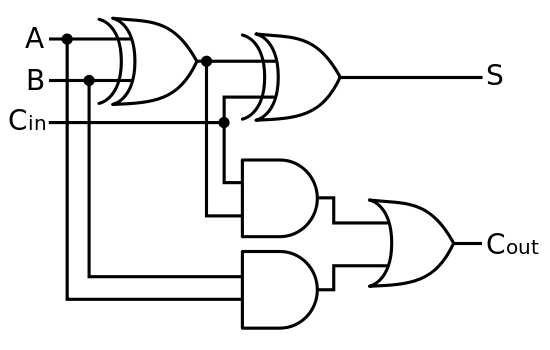
\includegraphics[width=\textwidth]{full-adder-circuit}

        \caption{Simple full adder circuit}
    \end{subfigure}%
    ~
    \begin{subfigure}[t]{0.5\textwidth}
        \centering
    % \begin{subfigure}
        % 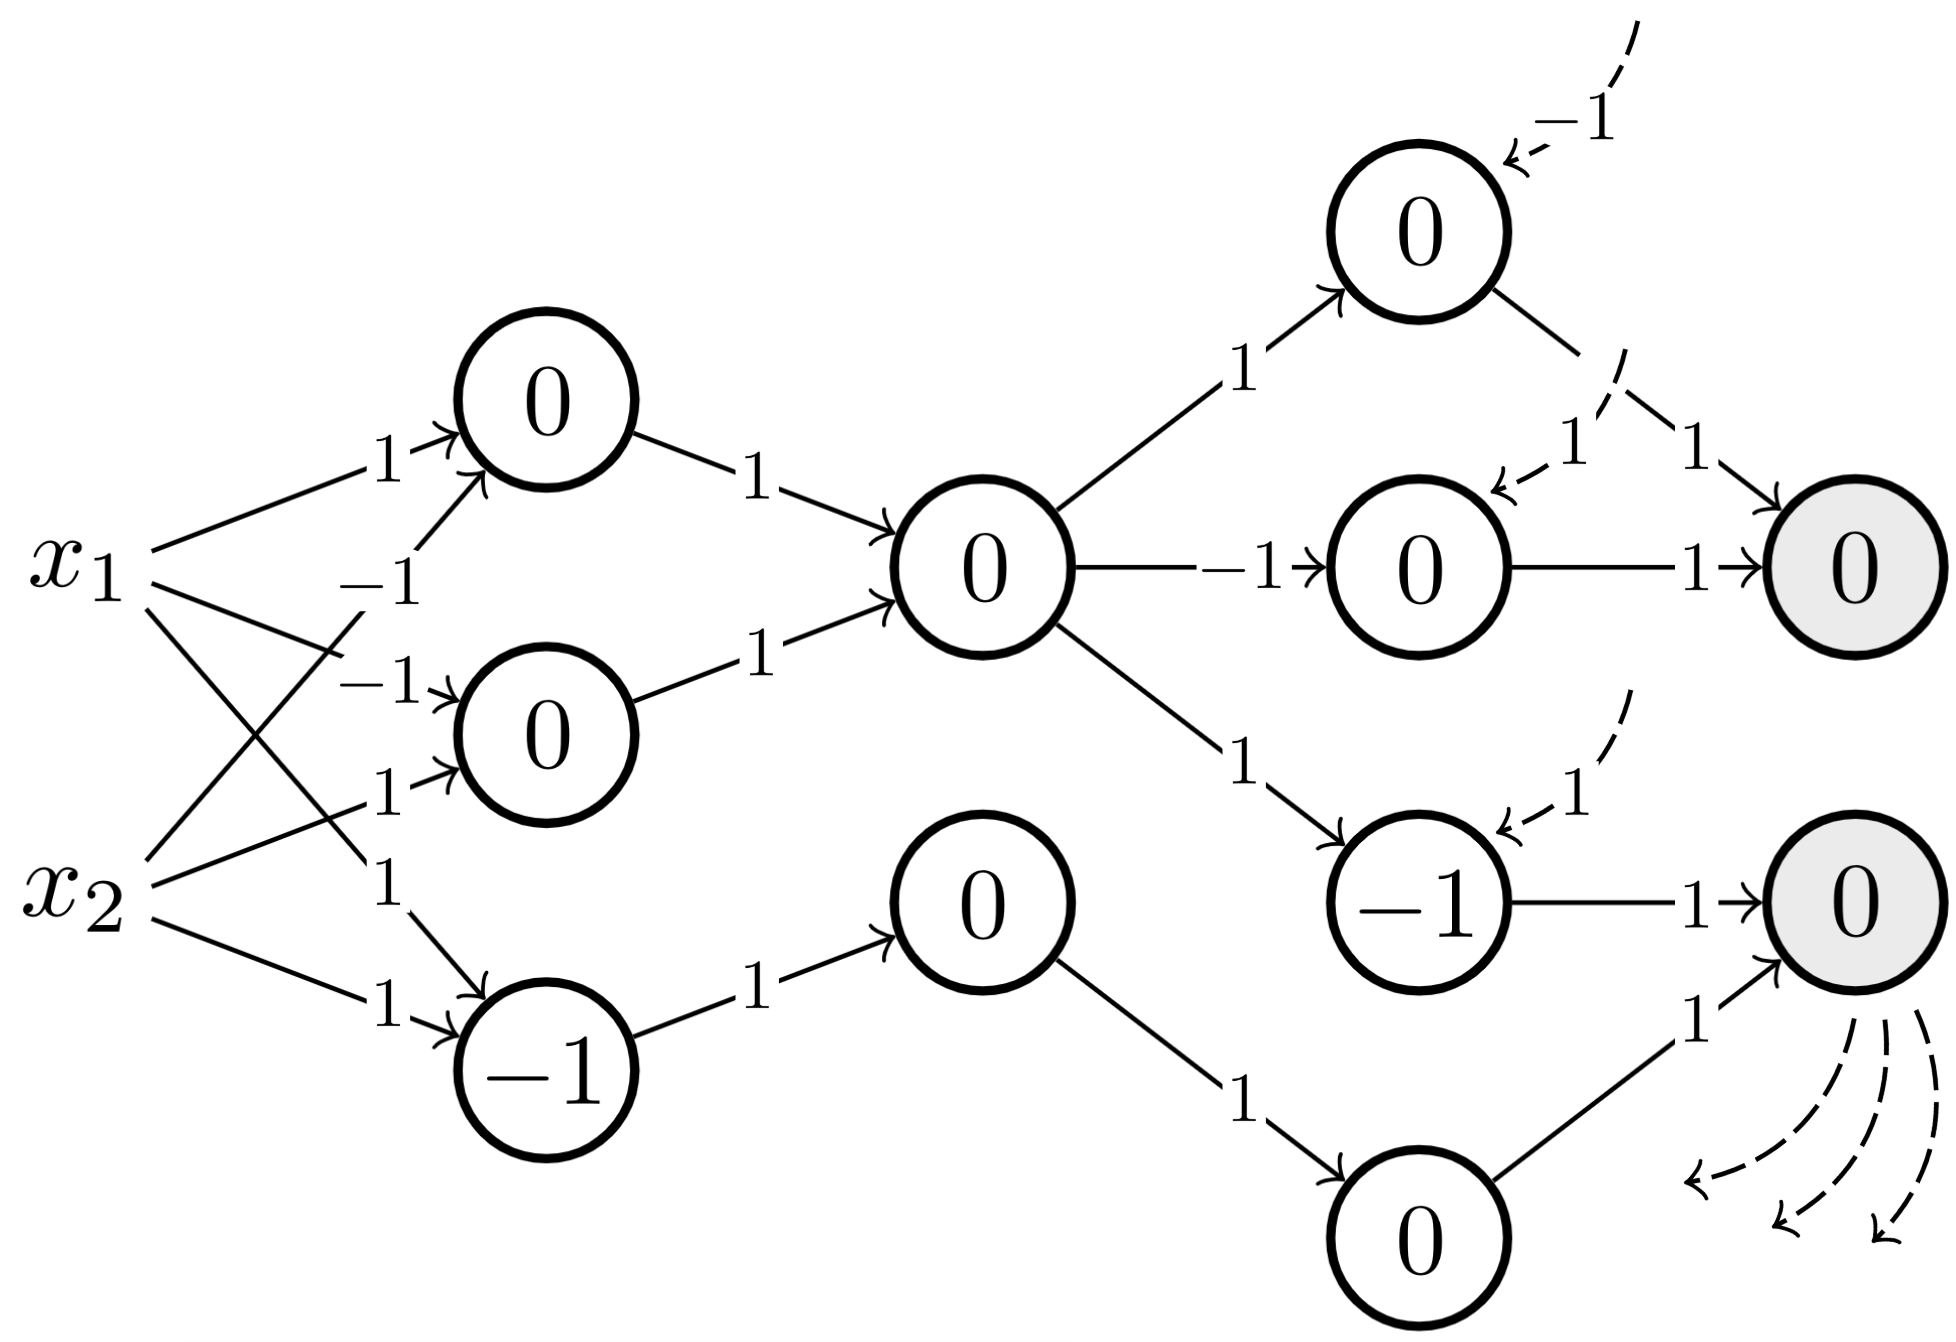
\includegraphics[width=\textwidth]{full-adder-ilrnn}
    % \end{subfigure}
    % \begin{tikzpicture}%[shorten >=1pt,->,draw=black!50, node distance=\layersep]
    %     \tikzstyle{every pin edge}=[<-,shorten <=1pt]
    %     \tikzstyle{neuron}=[circle,fill=black!25,minimum size=17pt,inner sep=0pt]
    %     \tikzstyle{input neuron}=[neuron, fill=green!50];
    %     \tikzstyle{output neuron}=[neuron, fill=red!50];
    %     \tikzstyle{hidden neuron}=[neuron, fill=blue!50];
    %     \tikzstyle{annot} = [text width=4em, text centered]
    
    %     % Draw the input layer nodes
    %     \foreach \name / \y in {1,...,4}
    %     % This is the same as writing \foreach \name / \y in {1/1,2/2,3/3,4/4}
    %         \node[input neuron, pin=left:Input \#\y] (I-\name) at (0,-\y) {};
    
    %     % Draw the hidden layer nodes
    %     \foreach \name / \y in {1,...,5}
    %         \path[yshift=0.5cm]
    %             node[hidden neuron] (H-\name) at (\layersep,-\y cm) {};
    
    %     % Draw the output layer node
    %     \node[output neuron,pin={[pin edge={->}]right:Output}, right of=H-3] (O) {};
    
    %     % Connect every node in the input layer with every node in the
    %     % hidden layer.
    %     \foreach \source in {1,...,4}
    %         \foreach \dest in {1,...,5}
    %             \path (I-\source) edge (H-\dest);
    
    %     % Connect every node in the hidden layer with the output layer
    %     \foreach \source in {1,...,5}
    %         \path (H-\source) edge (O);
    
    %     % Annotate the layers
    %     \node[annot,above of=H-1, node distance=1cm] (hl) {Hidden layer};
    %     \node[annot,left of=hl] {Input layer};
    %     \node[annot,right of=hl] {Output layer};
    % \end{tikzpicture}
    % \end{subfigure}

    %     \begin{circuitikz} 
    %     \draw
    %     (0,2) node[and port] (myand1) {}
    %     (0,0) node[and port] (myand2) {}
    %     (2,1) node[xnor port] (myxnor) {}
    %     (myand1.out) -- (myxnor.in 1)
    %     (myand2.out) -- (myxnor.in 2);
    %     \end{circuitikz}
        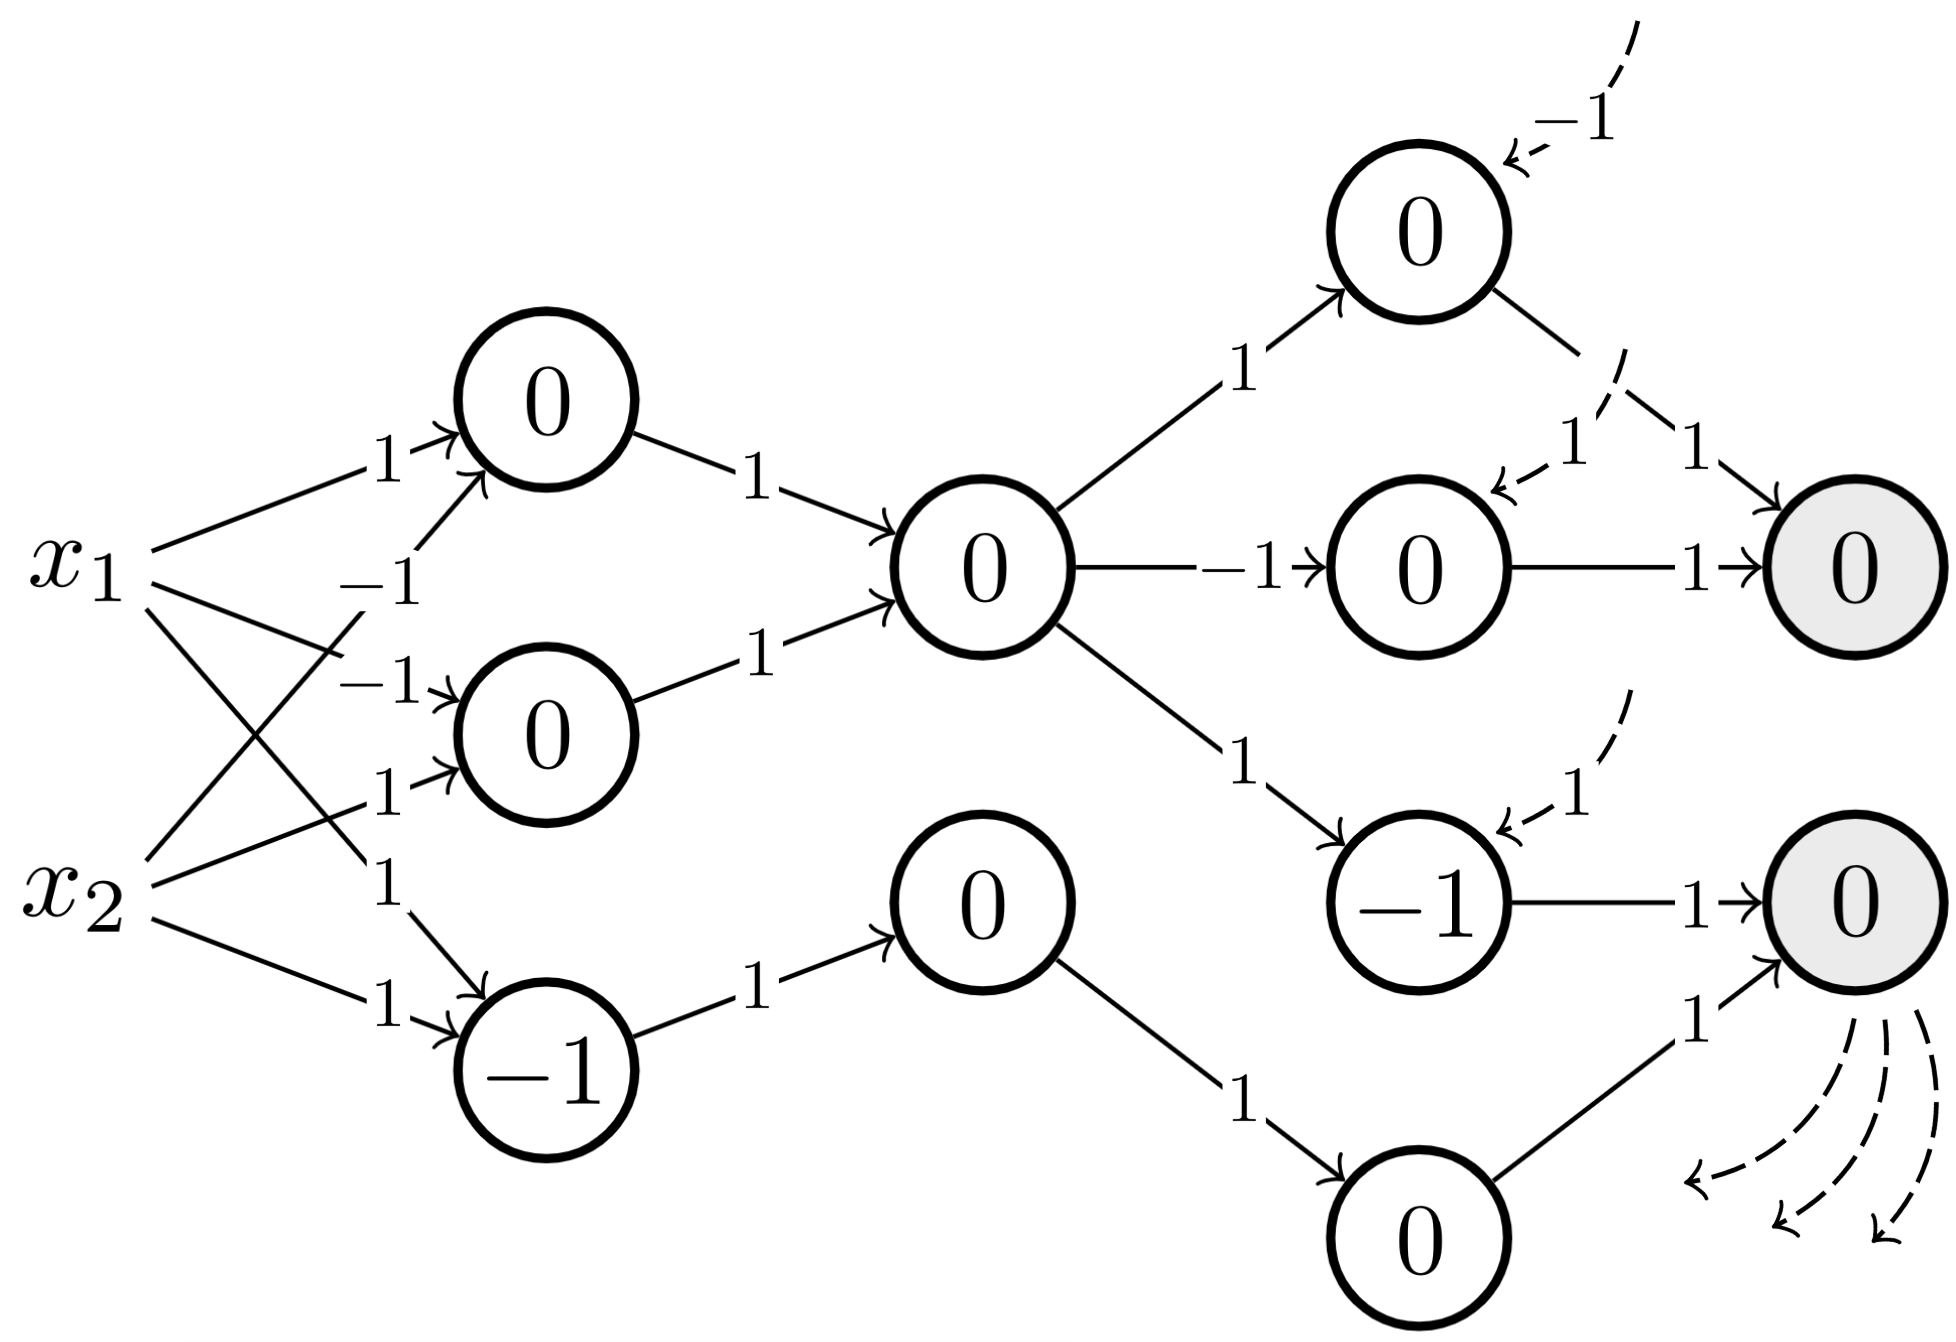
\includegraphics[width=\textwidth]{full-adder-ilrnn}
        \caption{Simple full adder ILRNN}
    %     \caption{Lorem ipsum, lorem ipsum,Lorem ipsum, lorem ipsum,Lorem ipsum}
    \end{subfigure}
    \caption{Full adder circuit and ILRNN equivalent}
    \label{fulladder}
\end{figure*}

\subsection{Manual construction}

A structure that solves the binary addition task is the full adder circuit commonly used in the arithmetic logic units of CPUs. It implements Boolean algebra using nothing but basic logic gates. It is well known that simple neural networks with one hidden layer and nonlinear activation functions can represent the XOR logic gate as well as all other basic logic gates. % (\hl{Jordan(?)}).

We use this fact to construct a baseline neural network of manually defined architecture and weight configuration that solves the task exactly. This proves that a ILRNN exists that expresses the full adder functionality. Note that this correspondence would not have been possible using a standard deep RNN, it was made possible through top-down recurrent connections across layers.

Figure~\ref{fulladder} depicts both the origin full adder microcircuit as well as its neural equivalent. The numbers on the visible connections (drawn as arrows) mark the respective weights for that connection. Missing connections can be regarded as having a weight of 0. The numbers within the hidden and output nodes resemble the biases chosen for these nodes. Dotted arrows indicate inter-layer recurrent connections (that pass on the potential carry). Only 3 recurrent connections are needed to reconstruct the full adder as a neural circuit. Note that for this weight configuration for ILRNN to work, the binary step needs to be chosen as activation. 

% \begin{itemize}
%     \item Note that this is more elegant than the full adder circuit because it needs one full adder circuit for every digit in the addends (no recurrence afaik?)
%     \item Note that the full adder (and more broadly, arithmetic logic units) are instantiations of \textit{combination logic} which according to Chomsky (XXX cite Chlomsky) are a class of automata less expressive than even finite state machines
% \end{itemize}

\subsection{Analytical solution}

When one considers a linear activation function (i.e. $f(x) = x$), the learning problem is reduced to a system of polynomials. Calculcating the Gr\"obner basis for this system expectedly returns 0 \cite{buchberger2006bruno}, signifying that there exists no solution. This is insofar expected, as the XOR gate alone requires a nonlinear activation function in order to be represented by a neural net. % (\hl{XXX}).

% \begin{itemize}
%     \item Firstly, we address the question: Does there exist a recurrent neural network that is able to perfectly solve / represent a perfect solution to the binary addition task? This we tried using analytical solutions first. +linear activation 
%     \item \textit{Do I mention my approach using Gr\"{o}bner bases here? Yes, also add some maths for it}
%     \item Since conventional learning algorithms are iterative / convex optimization, it is reasonable to ask whether the toy problem posed here can be solved analytically (\textit{This sentence doesn't make sense in itself yet because how do I jump from optimization to solving?}
%     \item \textit{Did I even do this on a proper architecture? Did I try this on the full adder architecture with linear activations?}
%     \item \textit{\hl{Can I say that there exists no solution to the simple deep RNN w/o inter-layer recurrent connections?}}
% \end{itemize}

\subsection{Learning / iterative optimization}

Finally, we regard the task as a supervised sequence learning problem and train the network using backpropagation through time (BPTT) \cite{rumelhart1986learning}. We tried a custom activation function used to resemble the binary outputs of the full adder microcircuit gates, for which we also implemented custom gradients following the work on binarized convolutional neural networks \cite{RastegariORF16,DBLP:journals/corr/CourbariauxB16}.
% \hl{Add math.}

Unfortunately, our attempts to train the resulting architecture using conventional methods did not lead to the desired results. Standard optimizers such as Adam with different learning rates, different activation functions employed in the network (binary step, ReLU, Sigmoid) converged to a suboptimal solution. Even initializing the weights to the target solution perturbed by small amounts of white noise would not converge as desired.

Bland publish a thorough analysis on the learning behavior and the error surface of the XOR function for a simple neural network (\citeyear{trove.nla.gov.au/work/18037125}). This is relevant here in the sense that the desired full adder consists of several XOR gates that should be learned. Bland finds that empirically only a small share of initial weight configurations converge to a solution computing XOR (\citeyear{trove.nla.gov.au/work/18037125}).

% \begin{itemize}
%     \item Show graph of accuracy over sequence length (how it slowly degrades for normal RNN) vs. how it stays at 100\% for manual solution / ILRNN (depending on what I can achieve here...)
%     \item \textit{Cite "Learning XOR - exploring the space of a classic problem"}
% \end{itemize}

% Note use of \abovespace and \belowspace to get reasonable spacing
% above and below tabular lines.

\section{Conclusion \& Future Work}

All in all, this paper introduces a new recurrent network architecture called ILRNN (iLearn) and a binary addition task that is used to evaluate it. While we find that the new architecture can express the exact solution, conventional training algorithms fail at finding it. The binary addition task seems like a good test bed for further research about exact learning in neural networks.

% Uncomment this
% \begin{itemize}
%     \item \hl{Come back to expressivity, learnability and interpretability}
%     \item In terms of interpretability, we have given an example of how single neurons or small groups of neurons can be interpreted to represent logic gates (following the tradition of the earliest researchers)
% \end{itemize}

So far, architecture was hand-crafted (and weights needed to be initialized close to hand-crafted solution?), which is far from practical. Possible extensions to address the witnessed learnability problems are the following:

\begin{itemize}
    \item The proposed network could be a sub-network of a larger network.
    \item Other (biologically inspired) learning algorithms could be tried out (f.e. differential plasticity, hebbian learning, local learning), new forms of regularization.
    \item Find a distributed representation of the logic gates also used in this paper
    \item It still needs to be evaluated how well the new architecture fares with larger problems and in combination with other recent deep learning-related refinements such as LSTM cells, regularization, bi-directionality etc.
    \item Regarding larger problems, those not requiring exact learning could be considered.
    \item Now that per-layer constraints in connectivity have been loosened, it would also be interesting to ask whether the law of synchrony of computation of neurons in artificial neural networks can be loosened.
\end{itemize}

% So far we have ausgelagert the problem of memory by feeding digits two at a time. Incorporate notions of memory (both internal and external to the neural core)

% The learning algorithm has no "intention"/"inclination" yet to learn the general solution

% Asynchronously firing neurons (ah well, currently its firing \textit{rates}, right?)


% We strongly encourage the publication of software and data with the
% camera-ready version of the paper whenever appropriate. This can be
% done by including a URL in the camera-ready copy. However, do not
% include URLs that reveal your institution or identity in your
% submission for review. Instead, provide an anonymous URL or upload
% the material as ``Supplementary Material'' into the CMT reviewing
% system. Note that reviewers are not required to look at this material
% when writing their review.

% Acknowledgements should only appear in the accepted version.
% \section*{Acknowledgements}

% \textbf{Do not} include acknowledgements in the initial version of
% the paper submitted for blind review.


% In the unusual situation where you want a paper to appear in the
% references without citing it in the main text, use \nocite
% \nocite{langley00}

\bibliography{ilrnn_icml19}
\bibliographystyle{icml2019}

\end{document}


% This document was modified from the file originally made available by
% Pat Langley and Andrea Danyluk for ICML-2K. This version was created
% by Iain Murray in 2018, and modified by Alexandre Bouchard in
% 2019. Previous contributors include Dan Roy, Lise Getoor and Tobias
% Scheffer, which was slightly modified from the 2010 version by
% Thorsten Joachims & Johannes Fuernkranz, slightly modified from the
% 2009 version by Kiri Wagstaff and Sam Roweis's 2008 version, which is
% slightly modified from Prasad Tadepalli's 2007 version which is a
% lightly changed version of the previous year's version by Andrew
% Moore, which was in turn edited from those of Kristian Kersting and
% Codrina Lauth. Alex Smola contributed to the algorithmic style files.
